\chapter{Collective communication, global data}

\section{Pass-on}

As can be seen in the following picture, the \textit{pass-on} method has been successfully implemented. For a better understanding of what is going on, the messages have been labelled with the rank of the sender. Thus, we can see that the value is correctly passed from a processor to its direct neighbor.
\begin{figure}[!h]
\begin{center}
	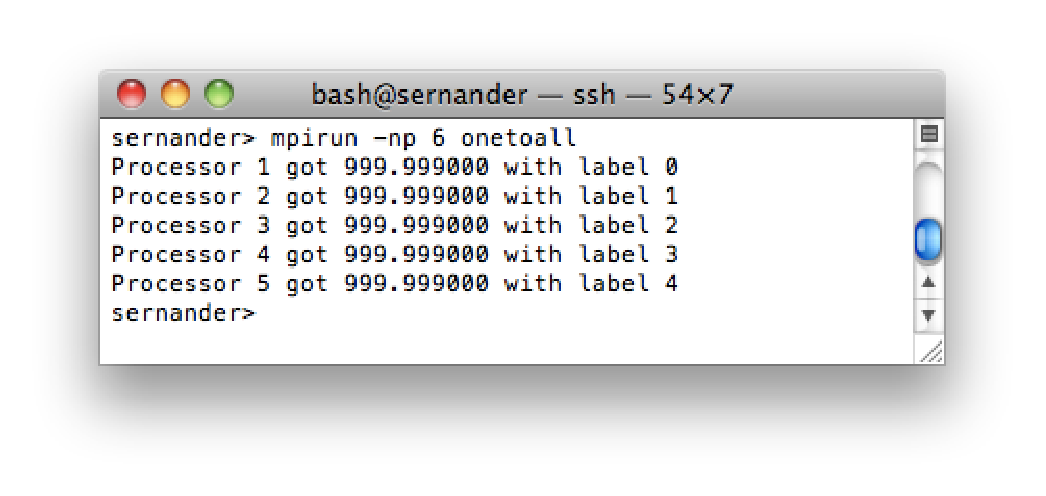
\includegraphics[width=\textwidth]{pic/passon.eps}
	\caption{Pass-on}
\end{center}
\end{figure}

\section{Fan-out}

Like the last version we print the rank of the sender. In this version we set the number of step with:
$$ceil(ln(NP))$$
where $NP$ is the total number of processor.

At each step we define the senders as:
$$S_{step}=\{\sqqs p, rank < 2^{step} \sand rank + 2^{step} < NP\}$$
where $p$ is a processor. This disallow processor who did not receive data to send, and processor who will send data to an non-existant processor.

Following the same principe we define the receivers as:
$$R_{step}=\{\sqqs p, rank < 2^{step+1} \sand rank - 2^{step} \ge 0\}$$
by using this, only processor that will receive a message at this step will fetch it message.\\

There is the output of our implementation:

\begin{verbatim}
Lain-ux@nyarlathothep:code > mpirun -np 8 a.out 
Processor 1 got 999.999000 from 0
Processor 2 got 999.999000 from 0
Processor 3 got 999.999000 from 1
Processor 4 got 999.999000 from 0
Processor 5 got 999.999000 from 1
Processor 6 got 999.999000 from 2
Processor 7 got 999.999000 from 3
\end{verbatim}

As we can see, not everybody send messages.

\section{Broadcast}

The following picture allows us to verify the correctness of the program using \textit{MPI\_Bcast}.
\begin{figure}[!h]
\begin{center}
	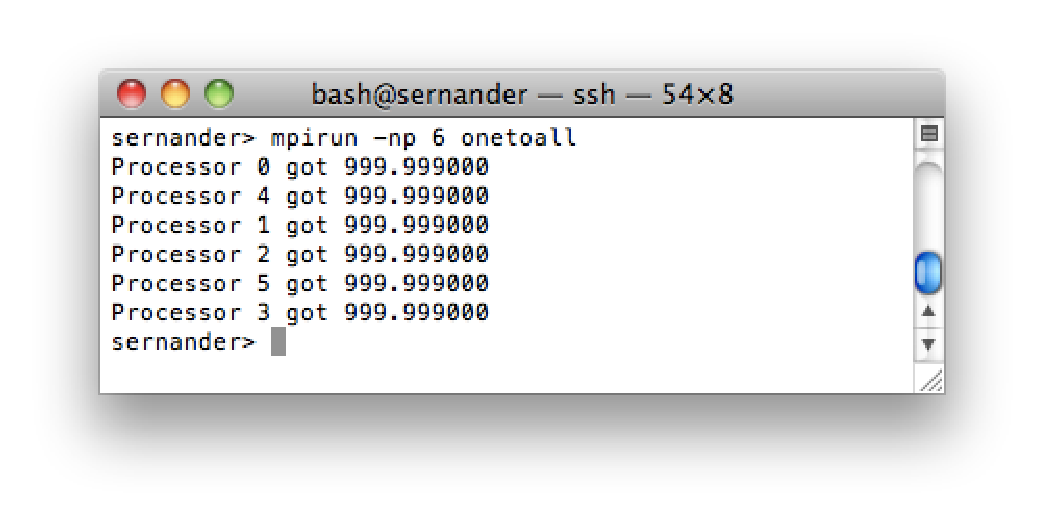
\includegraphics[width=\textwidth]{pic/bcast.eps}
	\caption{Broadcast}
\end{center}
\end{figure}

MPI does have a lot of other \textit{collective communication} operations, described as follows:

\begin{itemize}
	\item Barrier synchronization across all group members
	\item Broadcast from one member to all members of a group
	\item Gather data from all group members to one member 
	\item Scatter data from one member to all members of a group
	\item A variation on Gather where all members of the group receive the result
	\item Scatter/Gather data from all members to all members of a group
	\item Global reduction operations such as sum, max, min, or user-defined functions, where the result is returned to all group members and a variation where the result is returned to only one member (used in the following exercise) 
	\item A combined reduction and scatter operation
	\item Scan across all members of a group (also called prefix)
\end{itemize}
